\section{Interpretability Analysis}

% As for translating a single sentence the model performs multiple inferences, each one corresponding to a particular token predicted until reaching EOS, we capture different attention matrices as the sentence is generated. The size of the matrices resulting from cross and self-attention increase progressively as more tokens are predicted: we will have an attention score and value for each frame and previous token per prediction. To aggregate the attention across frames for each prediction step, we retain the maximum value from each row in the attention matrices corresponding to each subsequent token in the output sequence. We then apply \verb|min-max| normalization for visualization purposes.

\subsection{Decoder Cross-Attention}

We analyzed the cross-attention scores for the encoded frames when predicting each token. A higher attention score means that more information from that particular frame was used in the prediction of a token. Figure~\ref{subfig:decoder_ca_ex_1} shows the scores obtained during the translation of a complete sentence, where we can observe the following.

\begin{enumerate}
    
    \item The model does not pay attention to individual frames but rather to clusters of contiguous frames. This behavior is not typical of the attention mechanism in text to text models, but can be observed in tasks like audio transcription where these clusters correspond to a single target token~\cite{luo2020simplified}.

    \item The attention matrix seems to be shaped as a diagonal matrix, where the position of the predicted gloss in the sentence correlates with the part of the video the model is paying attention to: for the first glosses the model pays attention to the beginning of the video and, as we move forward through the sentence, the cluster of frames to which the models is paying attention moves forward as well.
    
\end{enumerate}

\begin{figure}[htb]
    \centering
    \begin{subfigure}[t]{.48\textwidth}
        \centering
        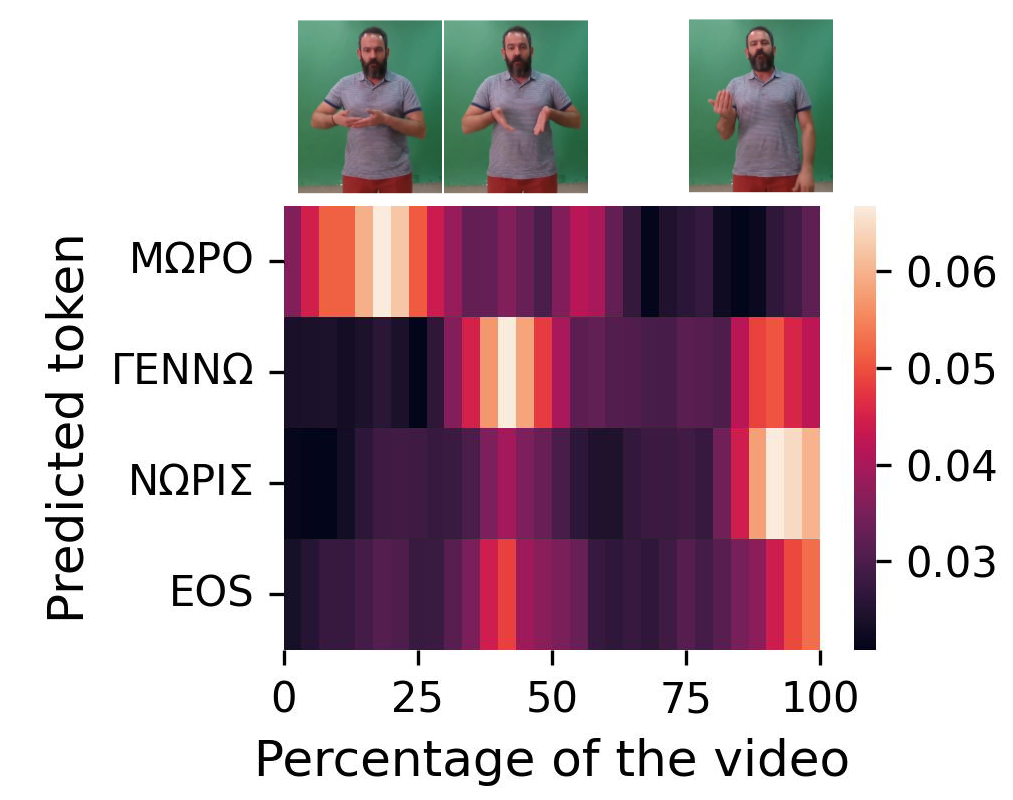
\includegraphics[width=\linewidth]{assets/examples/decoder_ca_heatmap_fh_layer0_idx509_with_frames.png}
        \caption{\textbf{Cross-attention scores across frames for each predicted token.} Above the heatmap, frames corresponding to the highest activation per gloss.}
        \label{subfig:decoder_ca_ex_1}
    \end{subfigure}\hfill
    \begin{subfigure}[t]{.48\textwidth}
        \centering
        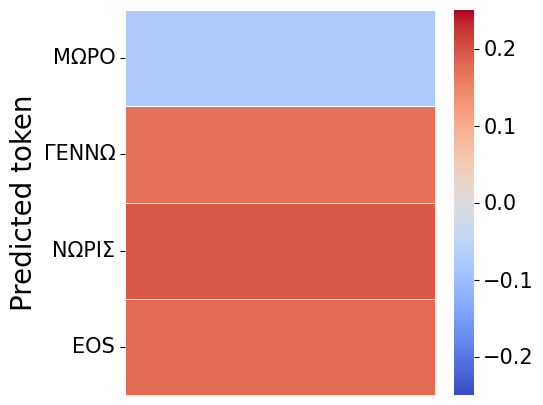
\includegraphics[width=.8\linewidth]{assets/examples/sa_ca_diff_gm_layer0_idx509.png}
        \caption{\textbf{Differences between self and cross-attention weights per inference.}}
        \label{subfig:sa_ca_diff_ex_1}
    \end{subfigure}
    \caption{Proposed interpretability methods applied to a single sample that translates to "ΜΩΡΟ ΓΕΝΝΩ ΝΩΡΙΣ" (BABY BIRTH EARLY).}
    \label{fig:single_sample_methods_vis}
\end{figure}

As glosses have a one-to-one relationship to the signs, these results suggest that the model actually identifies these signs in the video and the corresponding mapping to glosses. Frames shown above \ref{fig:decoder_ca_ex_1}, that correspond to the highest attention scores for the prediction of each gloss, support this conclusion, as they clearly correspond to the three different signs performed.

% \begin{figure}[htb]
%     \centering
%     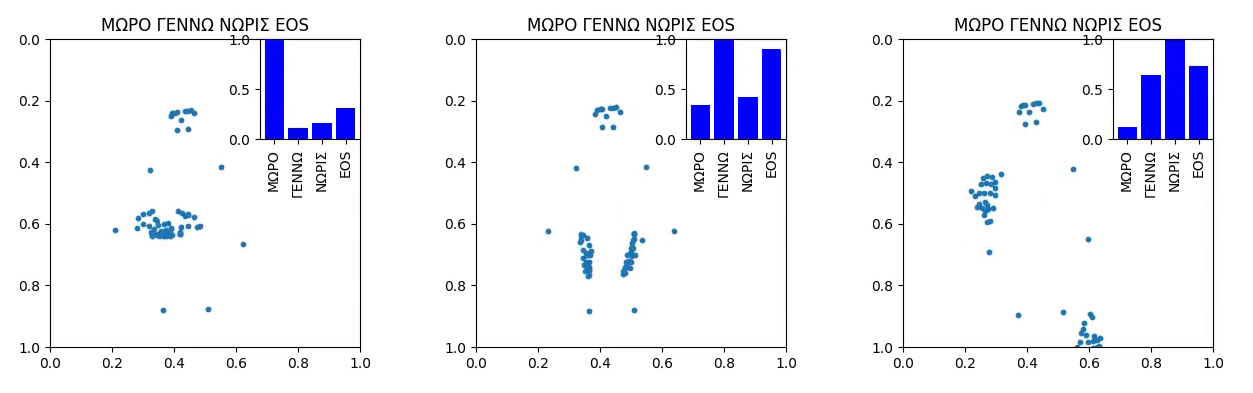
\includegraphics[width=0.8\linewidth]{assets/examples/decoder_ca_bars_fh_layer0_idx509.png}
%     \caption{Bar chart displaying the normalized attention values across the video sequence (frames 6, 13, and 28), illustrating how each bar reaches its maximum at the pose which is the most representative of the predicted token.}
%     \label{fig:decoder_ca_ex_1_bars}
% \end{figure}

\subsection{Self-Attention vs Cross-Attention}

In each decoding step, the cross-attention vector resulting from the previously analyzed scores for each frame, is combined with the self-attention vector by adding them to the embedding representation of each token. The vector with larger magnitude will be the one that adds more information to this new representation and thus to the prediction of the next token.

To understand the relative relevance of self and cross-attention for each prediction, we calculate the difference between the outputs of self-attention and cross-attention (averaged across the embedding dimensions). Positive values indicate a stronger contribution from the self-attention block (previous glosses), while negative values indicate a stronger contribution from the cross-attention block (the video poses).

Figure \ref{subfig:sa_ca_diff_ex_1} shows this difference for the prediction of each token of the same sentence shown in the previous example. It can be seen that as the model relies on video information for predicting the initial token, but for following predictions the self-attention has a greater influence.
